\documentclass[11pt]{article}
\usepackage[latin1]{inputenc}
\usepackage{amsmath}
\usepackage{amsfonts}
\usepackage{amssymb}
\usepackage{graphicx}
\usepackage{setspace}
\usepackage[left=1.00in, right=1.00in, top=1.00in, bottom=1.00in]{geometry}
\usepackage[english]{babel}
\newcommand{\forceindent}{\leavevmode{\parindent=1.5em\indent}} % em = roughly width of uppercase ``M", or just over a third of a cm

\usepackage{fancyhdr}

\pagestyle{fancy}
\fancyhf{}
\rhead{University of Houston $|$ Political Science}
\lhead{Learning \LaTeX: Week 5} %% BE SURE TO CHANGE THIS EACH WEEK
\rfoot{Page \thepage}

\usepackage[round]{natbib}
\bibliographystyle{apsr}

\begin{document}
	
	\title{Learning \LaTeX \\
		\vspace{1cm}
	\large Week 5: Presentations \& \texttt{Beamer}, pt. II \\ %% BE SURE TO CHANGE EACH WEEK
		\vspace{1cm}}
	\author{Philip D. Waggoner\footnote{{\texttt{philip.waggoner@gmail.com}}. This document was prepared by Philip Waggoner for the \textit{Weekly Workshops on Learning \LaTeX}, hosted by the Deparment of Political Science, University of Houston.}}
	\date{ } % getting rid of the automatic date
	\maketitle

\newpage

\tableofcontents

\newpage

\section{Introductory Remarks}
	
\forceindent With the basics of Beamer under our belts, let's shift to focus on how to mkae presentations more presentable, better formatted, and generally prettier. This week's workshop builds on last week's, assuming you are familiar with the basics of creating a presentation in \LaTeX\ using the Beamer documentclass. If you are not, then, reach out to me for last week's material. \\

\textbf{Our goals for today:}
\begin{itemize}
	\item Update, change and design Beamer presentations
	\item Include a Table of Contents
	\item Insert \& Use Blocks
\end{itemize}

\newpage

%%% GO OVER THEMES, packages, tables of contents, blocks, fancy stuff, and even powerdot and/or fancy slides for comparisons and extensions

\section{Design \& Themes}

\forceindent To make a nice looking, presentable presentation in Beamer, we have two options: 1. we can either manually change the formatting, or 2. we can use ``themes." As this is an introductory workshop, let's stick with the simplest approach of using prepackage themes that folks have already done the hard work of making consistent and nice.  \\

As such, we will need some new code to add to our preamble. Specifically, we need two new commands, ``mode" and ``usetheme." The mode command is accompanied by the word presentation as well as a set of braces, into which the usetheme command will be placed. Essentially, this combination of commands in the preamble tells \LaTeX\ that we are working with a presentation and want to access a pre-packaged theme for our presentation. It will then automatically provide colors and unique frame design. \\

Importantly, there are \textit{many} theme options to choose from. For a full list, visit, \linebreak{\texttt{http://deic.uab.es/~iblanes/beamer\_gallery/}}. We will only use a few for our cases today. Let's launch with my personal favorite for a variety of reasons: ``CambridgeUS." \\

So let's start with the following addition to our preamble:

\begin{figure}[!h]
	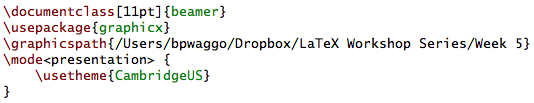
\includegraphics[scale=.5]{CODE1}
	\centering
\end{figure}

Make sure you change the graphicspath to be the location where you main document is stored. \\

Now, with our preamble properly specified, let's create a simple title slide using the CambridgeUS theme. Let's start with the following code:

\begin{figure}[!h]
	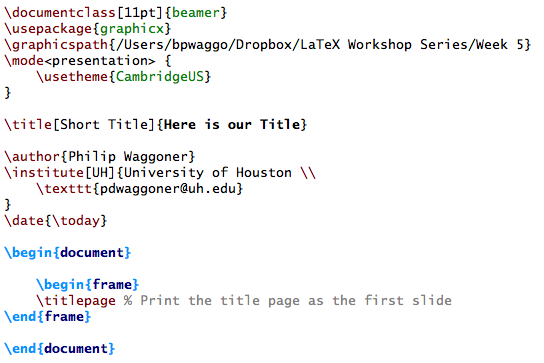
\includegraphics[scale=.5]{CODE2}
	\centering
\end{figure}

This now gives use the following title slide using the base color scheme in the CambridgeUS theme, as well as the basic frame foramtting (we will address more formatting below):

\begin{figure}[!h]
	
\includegraphics[scale=.5]{OUT2}
	\centering
\end{figure}

\newpage

Let's see another major theme, ``Berkeley." So let's update our original code by only changing the theme. \textit{Leave everything else the same to make a direct comparison}. Start with:

\begin{figure}[!h]
	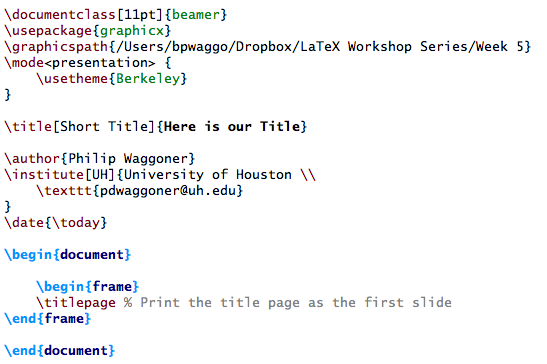
\includegraphics[scale=.5]{CODE3}
	\centering
\end{figure}

And this gives us the same information but on a completely differently formatted frame,

\begin{figure}[!h]
	
\includegraphics[scale=.5]{OUT3}
	\centering
\end{figure}

\newpage

\subsection{Color Themes}

\forceindent Importantly, within a theme, you can also change the color theme if you like the general layout of a theme, but don't like the colors. To do so, we add the new command, ``usecolortheme" to our preamble \textit{below} the theme command. So to update our original example using the Berkeley theme, let's use the ``crane" color theme:

\begin{figure}[!h]
	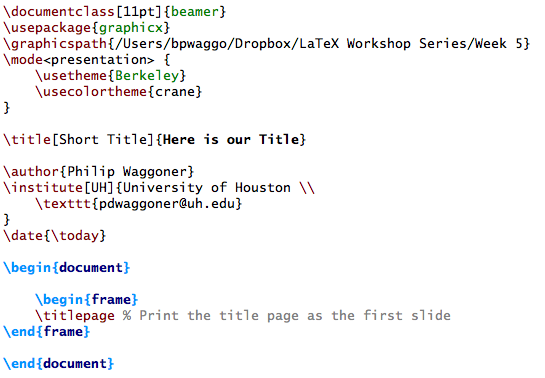
\includegraphics[scale=.5]{CODE4}
	\centering
\end{figure}

And this gives us a new frame with a new color scheme,

\begin{figure}[!h]
	
\includegraphics[scale=.5]{OUT4}
	\centering
\end{figure}

\newpage

Refer to the website above to see a full list of pre-programmed color themes. Note, the same process should be followed for different font themes. See the above website for a full list of those as well. 

\newpage

\section{Table of Contents}

\forceindent Tables of contents can be quite useful in Beamer presentations to provide signposts for the audience, as well as help you stay organized as you create the presentation. It is straightforward to insert a table of contents. To do so, we create a new frame with the command ``tableofcontents." This adds a table of contents automatically, based on the sections and subsections in your presentation. \\

Importantly, there are two main caveates in using a table of contents. First, you must be using the ``section" command as you would in a document. And second, you must be using a theme that is compatible with the table of contents. Some themes do not include these, but some do. So the first thing to check if you don't see a table of contents when you told it to be included, is the theme you are using. Try another them as a baseline troubleshooting step. \\

With that, let's see how this works. Start with the following code updating to use the ``Hannover" theme,

\begin{figure}[!h]
	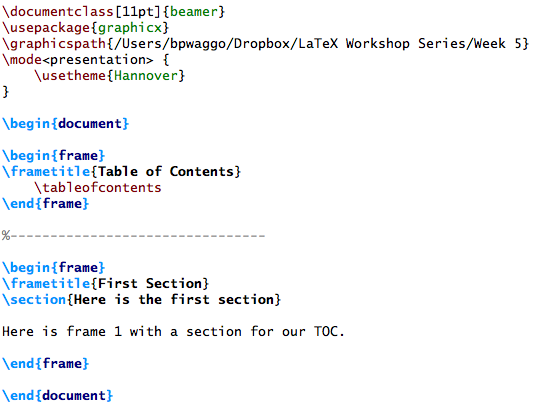
\includegraphics[scale=.5]{CODE5}
	\centering
\end{figure}

And see our output,

\begin{figure}[!h]
	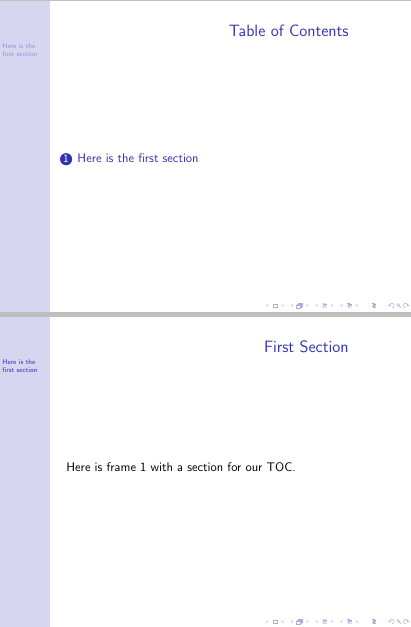
\includegraphics[scale=.5]{OUT5}
	\centering
\end{figure}

\newpage

Note a few things: we dropped out title frame for the sake of space, the frame title shows up on the leftside column, and when we get to the specific frame in the presentation, the text automatically gets darker.  Feel free to explore and try other themes and colorthemes. 


\newpage

\section{Inserting Blocks}

\forceindent A cool feature of Beamer and \LaTeX\ presentations is adding a block to highlight something in a different way (e.g., hypotheses, equations, etc.). Different colors are associated with different blocks, dependning on the needs. As a quick caveate, similar to the table of contents, some templates allow blocks (or have different colors and formatting associated with different blocks) and others don't. As with table of contents, if your typesetting doesn't include what you thought it should, start by trying another template to see if this fixes the problem. If need be, you can always resort to \texttt{Share Latex} or \texttt{Stack Exchange}. \\
	
There are several ways to add blocks. We can just use the ``block" environment (e.g., begin and end). We could also use the ``examples" environment to get a different color pre-formatted to stand out from our text. Or we could also use the ``alertblock" environment to make the color red. Note that using the base ``alert" command will turn any associated text red. The same is true for the blocks and the ``alertblock" environment specifically. To add these and get a sense of the differences, start with the following code using two different environments to see the differences in how the base themes format blocks differently. Type, \\

\begin{figure}[!h]
	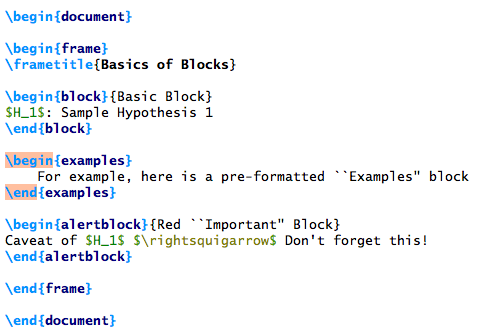
\includegraphics[scale=.5]{CODE6}
	\centering
\end{figure}

Using the ``Madrid" theme first, we see the colors are intense and the blocks are clearly separated from the rest of the frame as well as from each other,

\begin{figure}[!h]
	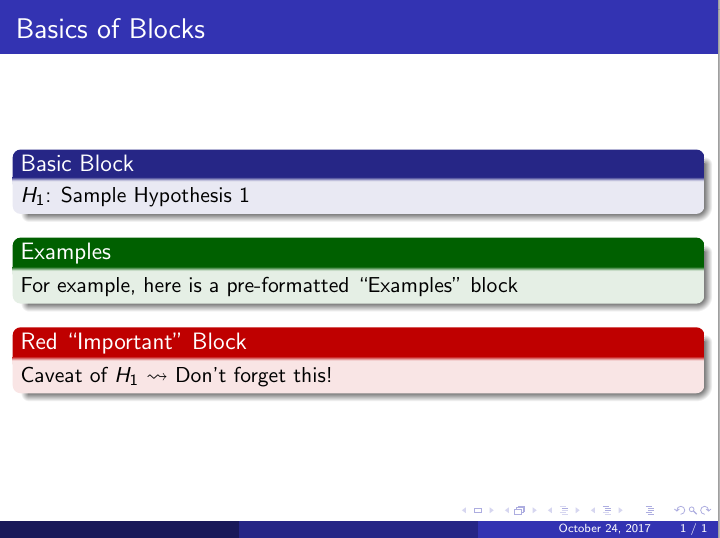
\includegraphics[scale=.5]{OUT61}
	\centering
\end{figure}

\newpage

But if we change the theme back to our original ``CambridgeUS" theme, we see the blocks, though still clearly fromatted, are a bit more subtle and blending in with the frame a bit more,

\begin{figure}[!h]
	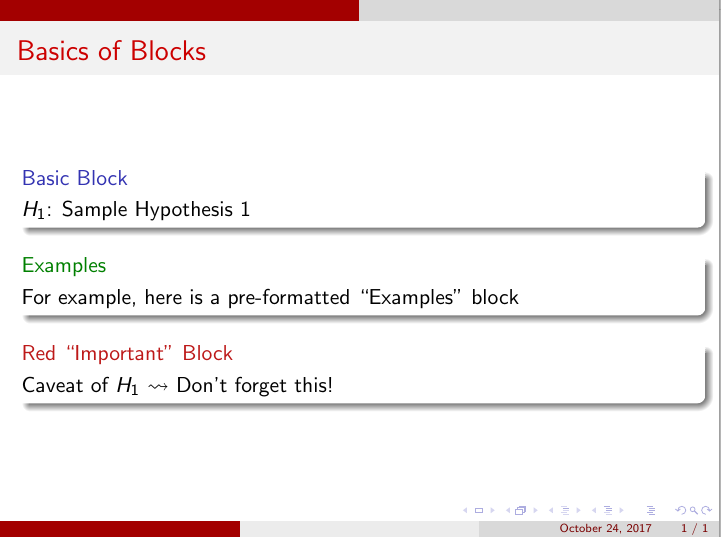
\includegraphics[scale=.5]{OUT62}
	\centering
\end{figure}

\newpage

\section{Miscellanea \& Final Words}

\forceindent As a final word, there are a few additional simple commands to allow you a little more flexibility to customizing your Beamer presentations. We will look at only three, though there are many more ways to customize your presentation. Include the following commands within the ``mode" command braces in your preamble (remember to include the backslash as the command operator): \\
\begin{itemize}
	\item Remove navigation symbols $\rightsquigarrow$ ``setbeamertemplate\{navigation symbols\}\{ \}"
	\item Remove the footer line in all frames $\rightsquigarrow$ ``setbeamertemplate\{footline\}"
	\item Include only a frame count at the bottom $\rightsquigarrow$ ``setbeamertemplate\{footline\}[page]" \\
\end{itemize}

I hope this soft introduction to Beamer has been useful, and that you feel confident to make well-formatted, good looking presentations using \LaTeX. As always, there are so many resources online. Starting with a simple Google search is always a good place to begin looking for additional updates, designs, templates, customizations, and so on.

\end{document}
